%!TEX root =  main.tex
\section{Introduction}


\begin{figure*}[ht!]
  \centering
  \begin{subfigure}[b]{0.45\textwidth}
    \centering
    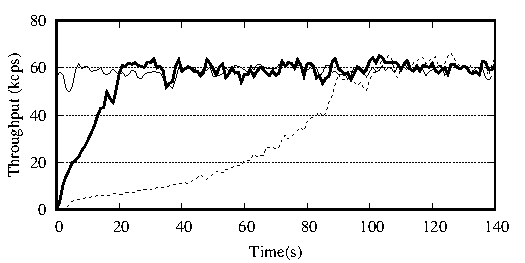
\includegraphics[width=0.95\columnwidth]{figures/experiments/dynastar-vs-dssmr-4p-0-tp}
    \caption{Throughput with strong locality}
  \end{subfigure}
  \begin{subfigure}[b]{0.45\textwidth}
    \centering
    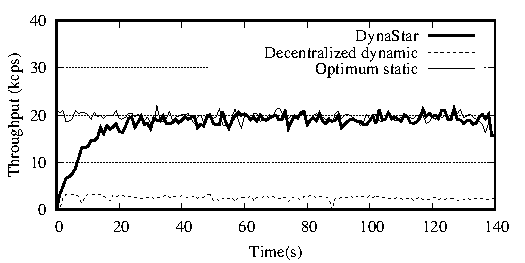
\includegraphics[width=0.95\columnwidth]{figures/experiments/dynastar-vs-dssmr-4p-5-tp}
    \caption{Throughput with weak locality}
  \end{subfigure} \\
  \begin{subfigure}[b]{0.45\textwidth}
    \centering
    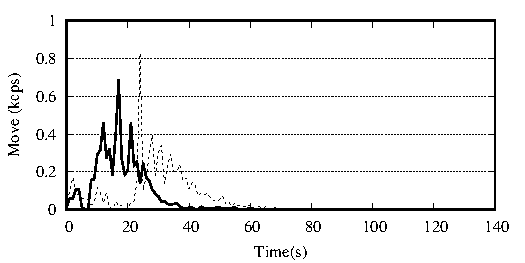
\includegraphics[width=0.95\columnwidth]{figures/experiments/dynastar-vs-dssmr-4p-0-move}
  \caption{Number of move commands with strong locality}
  \end{subfigure}
  \begin{subfigure}[b]{0.45\textwidth}
    \centering
    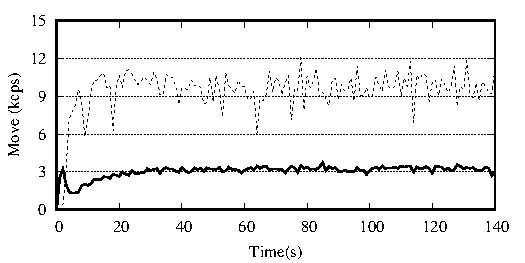
\includegraphics[width=0.95\columnwidth]{figures/experiments/dynastar-vs-dssmr-4p-5-move}
    \caption{Number of move commands with weak locality}
  \end{subfigure}
  \caption{\dynastar, optimum static and decentralized dynamic schemes under strong and weak locality (4 partitions).}
  \label{fig:motivation}
\end{figure*}




State machine replication (SMR) is a fundamental technique for
building fault-tolerant systems and services. With SMR, state is
replicated on a set of servers and each replica deterministically
executes the same sequence of client commands in order to maintain
consistency~\cite{Lam78,Sch90}. Unfortunately, classic state machine replication does not
scale, since each replica must execute every command. In order to
improve the scalability of SMR, several systems have investigated the
use of state partitioning~(e.g., \cite{corbett2013spanner, bezerra2014ssmr,Glendenning:2011kj,
  Aguilera:2007,bli16edcc}).

In principle, increasing the number of partitions should result in
increased system performance. However, if the execution of commands involves
multiple partitions, then performance can
actually decrease, due to overhead from ordering and coordinating
commands across partitions to ensure strong consistency. Moreover, if
data is not distributed carefully, then load imbalances can nullify
the benefits of partitioning. Thus, an ideal partitioning scheme is
one that would both (i) allow commands to be executed at a single
partition only, and (ii) evenly distribute data so that load is
balanced among partitions.  We refer to workloads that can be
partitioned in a way that satisfies these two properties as exhibiting
\emph{strong locality}.

Broadly speaking, there are two classes of techniques for
partitioning: \emph{static} and \emph{dynamic}.
Figure~\ref{fig:motivation} shows the result of a motivating
experiment that compares two representative systems, one of each class. In the
experiment, we measured the throughput and number of state moves over
time with two different workloads: one with strong locality and one
with weak locality. The workloads are inspired by the social network
Twitter, in which the network is modeled as a graph, and users can
``post'' messages. The social graph was generated using a Zipfian
distribution, where the Zipf parameter was adjusted to alter the
locality.  For brevity, we postpone the details of the experimental
setup until Section~\ref{sec:experiments}.


Static techniques choose an immutable assignment of application state variables to partitions
prior to executing commands. As an example of a static approach for
use in the experiment, we modified the S-SMR
system~\cite{bezerra2014ssmr} to use the static
METIS~\cite{Abou-Rjeili:2006} partitioning algorithm.  The METIS
algorithm is optimized to minimize edge-cuts when partitioning a
static social graph. 
In the workload with strong locality, METIS partitions the social graph such that all posts are single partition;
in the workload with weak locality, although most commands are single partition, a small fraction of posts involves multiple partitions.
As expected, we see that the throughput is less
for the weak locality workload, due to the more expensive execution of multi-partition posts.
%since the static scheme incurs overhead when accessing multiple partitions to execute commands.
For workloads that do not change the graph structure, the
results in Figure~\ref{fig:motivation} show a theoretical optimal
throughput.  Of course, these results are not achievable in practice,
since for real workloads, the graph would change over time (e.g., in
social networks users join and leave the system, connections are
created and removed).


Dynamic techniques address the limitations of static techniques by adapting
the partitioning scheme as workloads change.  
For example, a dynamic technique can move data ``on demand'' to maximize the number of single partition user commands, while avoiding imbalances in the load of the partitions.  
%Typically, this is
%implemented by moving data ``on demand'' to a single partition which
%executes a user command.  
The major challenge in designing a dynamic
scheme is determining how the system selects the partition to which to
move data.
%
The second system in Figure~\ref{fig:motivation} evaluates the dynamic
partitioning strategy implemented by the DS-SMR system~\cite{hoang2016}.
DS-SMR selects partitions randomly. This allows for a completely 
decentralized implementation, in which partitions make only local
choices about data movement.  We refer to this approach as
\emph{decentralized dynamic}.  As Figure~\ref{fig:motivation} shows,
the {decentralized dynamic approach works well for data with strong
  locality, but is unstable for workloads with weak locality, since
  data is constantly moved from one partition to another.


In this paper, we introduce \dynastar, a new dynamic approach to the
state partitioning problem.  Like other dynamic approaches, \dynastar
does not require any a priori knowledge about the workload. However,
\dynastar differs from prior approaches because it maintains a
centralized, global view of the network.  \dynastar minimizes the
number of state relocations by monitoring the workload, and
re-computing an optimal partitioning on demand using a static
partitioning algorithm.  As a preview of our results,
Figure~\ref{fig:motivation} also includes measurements for \dynastar.
We see that \dynastar is able to achieve throughputs comparable to
the optimal static scheme, while adapting to workload changes
on-the-fly, and preserving strong consistency.


With \dynastar, a location oracle maintains two data structures: (i) a
mapping of application state variables to partitions, and (ii) a \emph{workload graph}
with state variables as vertices and edges as commands that access the
variables.  When a client submits a command, it must first contact the
location oracle to discover the partitions on which state variables are
stored.  If the command accesses variables in multiple partitions, the
oracle issues a move command to the partitions, re-locating variables to
a single partition. Of course, when re-locating a variable, the oracle
is faced with a choice of which partition to use as a destination.
\dynastar chooses the partition for relocation (i.e., one that
would minimize the number of state relocations) by partitioning the
workload graph using the METIS partitioner.
Although METIS does not necessarily produce the best possible partitioning of the workload graph, it offers a good compromise between performance and partitioning quality.

\dynastar implements the oracle as a regular partition, replicated in a set of nodes, to tolerate failures.
To ensure that the oracle does not become a performance bottleneck, clients can cache location information.
Therefore, clients only query the oracle when they access a variable for the first time or when cached entries become invalid (i.e., because a variable changed location).
\dynastar copes with commands addressed to wrong partitions by telling clients to retry a command.

%\rjs{Should we say something about the location oracle not being a bottleneck?}

We have fully implemented \dynastar and compared its performance to
the dynamic partitioning protocol proposed by Long et
al.~\cite{hoang2016} and to the optimized static partitioning scheme.
%Our prototype can handle workload graphs with half a million variables
%and tens of millions of connections. \ef{Not yet :-|}
In workloads that present strong
locality, all three protocols eventually delivered comparable
performance, although \dynastar converged more quickly than the
decentralized scheme.  In workloads with weak locality, however,
\dynastar largely outperformed the decentralized scheme and performed
similar to the optimized static partitioning scheme.

%The reason for the surprisingly high performance of \dynastar compared to the optimized
%static partitioning scheme is that 
%\textbf{we need to explain this!!!
%:-)} \ef{If the cost of migrating the object outperforms the cost of 
%signaling partitions, why performance get similar when we have more partitions?} 
%\lle{in static scheme, partitions exchange signal in every global commands,
%while, in dynamic scheme, there is chance that partitions already have
%data, thus no communication needed. More over, signaling is a two-way mechanism,
%while moving objects in dynamic scheme is only one-way, which leads to less data
%is being exchanged}

The paper makes the following contributions:
\begin{itemize}
\item It introduces \dynastar and discusses its implementation. 
\item It evaluates different partitioning schemes for state machine replication under a variety of conditions.
\item It describes \appname{} to demonstrate how \libname{} can be used to implement a scalable social network service.
\item It presents a detailed experimental evaluation of \dynastar
%including real social network graphs with half a million users and 14 million edges.
\end{itemize}

The rest of the paper is structured as follows.
Section~\ref{sec:sysmodel} presents the system model.
Section~\ref{sec:background} reviews existing scalable state machine replication approaches.
Section~\ref{sec:dynastar} introduces \dynastar, describes the technique in detail and argues about its correctness.
Section~\ref{sec:implementation} overviews our prototype.
Section~\ref{sec:experiments} reports on the results of our experiments.
Section~\ref{sec:rw} surveys related work and
Section~\ref{sec:conclusion} concludes the paper.




%% %% Because single-partition commands are much more efficient than
%% %% multi-partition commands (i.e., in some cases by a factor of more than
%% %% 10x), the performance of a distributed storage system is particularly sensitive to the way
%% %% the service state is partitioned.


%% \subsection{State Machine Replication}

%% State machine replication (SMR) is a well-established technique to
%% develop highly available services (e.g.,
%% \cite{Shvachko:2003,Ghemawat:2003,Burrows:2006,MacCormick:2004}).  In
%% essence, the idea is that replicas deterministically execute the same
%% sequence of client commands in the same order and in doing so traverse
%% the same sequence of states and produce the same results.  State
%% machine replication provides configurable fault tolerance in the sense
%% that the system can be set to tolerate any number of faulty replicas.
%% Increasing the number of replicas, however, will not scale performance
%% since each replica must execute every command.  Unfortunately,
%% increasing the number of replicas will not scale performance since
%% each replica must execute every command.

%% S-SMR relies on an atomic multicast primitive to consistently order
%% commands within and across partitions.  Commands that access objects
%% located in a single partition (i.e., single-partition commands) are
%% multicast to the concerned partition and executed like in classical
%% SMR.  Commands that access objects located in multiple partitions
%% (i.e., multi-partition commands) are multicast to all involved
%% partitions.  To prevent command interleaves that violate strong
%% consistency, partitions coordinate during the execution of
%% multi-partition commands.



%% \subsection{Motivating Example}
